\documentclass[10pt, oneside]{article}   	% use "amsart" instead of "article" for AMSLaTeX format
\usepackage{geometry}                		% See geometry.pdf to learn the layout options. There are lots.
\geometry{a4paper}                   		% ... or a4paper or a5paper or ... 
%\geometry{landscape}                		% Activate for rotated page geometry
%\usepackage[parfill]{parskip}    		% Activate to begin paragraphs with an empty line rather than an indent
\usepackage{graphicx}				% Use pdf, png, jpg, or eps§ with pdflatex; use eps in DVI mode
								% TeX will automatically convert eps --> pdf in pdflatex		
\usepackage{float}	
\usepackage{url}						
\usepackage{amssymb}

%SetFonts

%SetFonts


\title{Simulated Irritable Bowel Syndrome (IBS) study}
\author{Driven by prompting ChatGPT-4 and DALL$\cdot$E 3}
\date{\footnotesize [Input by Arvid Lundervold to the PLEN-04 Debate at PCBBE-2023]}							% Activate to display a given date or no date

\begin{document}
\maketitle

\begin{center}

\includegraphics[width=0.25\textwidth]{pcbbe-debate-dalle-fig-ibs.png}

{\scriptsize \url{https://github.com/arvidl/PCBBE-2023-explore}}
\end{center}


\section{Methods}

\subsection{Data Preprocessing}
The dataset was initially structured for a regression problem, aiming to predict the variable \textit{Post\_IBS\_Symptoms} based on a set of features. To adapt this for a classification problem, the \textit{Post\_IBS\_Symptoms} were categorized into three equi-probable classes: Low, Medium, and High. This categorization was based on quantiles, ensuring that each class contained an approximately equal number of instances.

\subsection{Feature Selection}
For the classification task, the features selected included \textit{Baseline\_IBS\_Symptoms}, \textit{Baseline\_Stress\_Level}, and \textit{Baseline\_Microbiota\_Diversity}.

\subsection{Model Training}
A Random Forest Classifier was employed for the classification task. The model was trained with 100 estimators and utilized a random state of 42 for reproducibility. The dataset was randomly partitioned into training and testing sets, with 80\% of the data used for training and the remaining 20\% for testing.

\subsection{Evaluation Metrics}
The performance of the model was assessed using a confusion matrix and derived metrics such as precision, recall, and F1-score for each class. These metrics offer a comprehensive evaluation of the model's capability to correctly classify instances into the three predefined classes.

\section{Results and Interpretation}

\subsection{Confusion Matrix}
The confusion matrix indicated that the model had varying degrees of success in classifying instances into the three classes. It performed well in identifying the 'Low' and 'High' symptom levels but faced challenges in accurately classifying the 'Medium' level.

\begin{figure}[H]
   \centering
   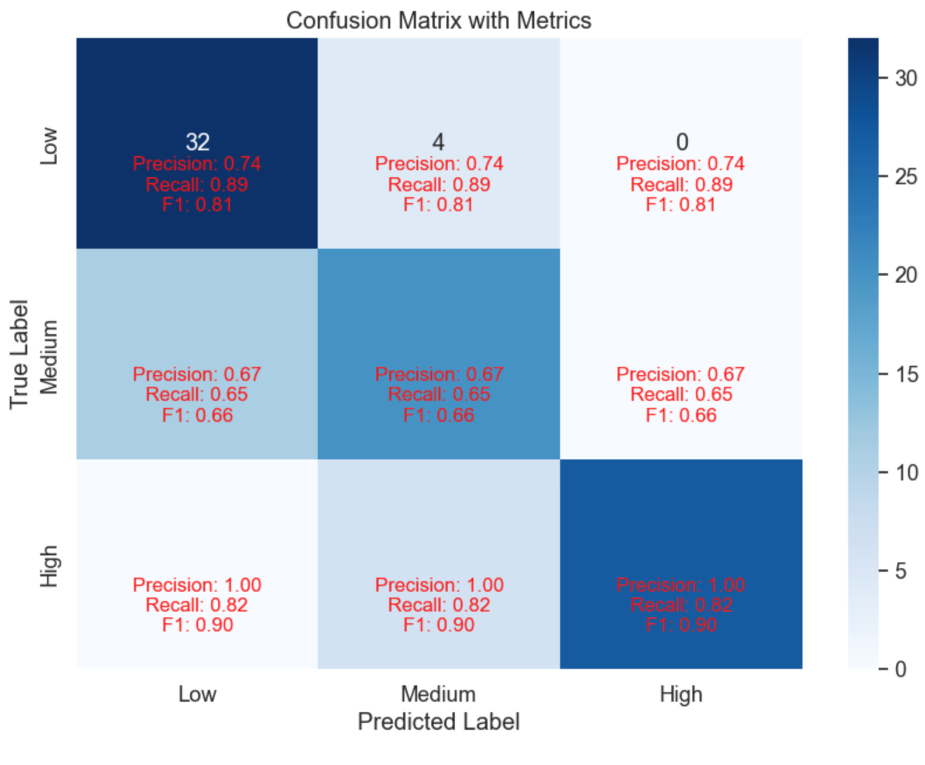
\includegraphics[width=0.60\textwidth]{res_14.png} % requires the graphicx package
   \caption{The confusion matrix (from {\tt 03-ibs-simstudy.ipynb})}
   \label{fig:isb-cm}
\end{figure}

\subsection{Precision, Recall, and F1-score}
The model exhibited high precision and recall for the 'Low Symptoms' class, indicating a strong ability to correctly identify and not overlook instances of low symptom levels. For the 'Medium Symptoms' class, both precision and recall were moderate, suggesting that the model had some difficulty in distinguishing medium symptom levels from the low and high levels. In the case of the 'High Symptoms' class, the model showed high precision but moderate recall, implying that while it was proficient at correctly identifying high symptom levels, it did miss some instances.

\subsection{Overall Assessment}
The Random Forest Classifier demonstrated a robust capability to classify instances into the 'Low' and 'High' symptom levels but encountered challenges with the 'Medium' level. This could be attributed to overlapping features between the 'Medium' and the other classes, which may require further investigation for feature engineering or selection. In summary, the model is promising but could benefit from additional tuning and possibly the inclusion of more features to enhance its performance, particularly for the 'Medium' class.


\end{document}  
